\documentclass{beamer}
 
\usepackage[utf8]{inputenc}
\usetheme{Warsaw}
\usecolortheme{beaver}
 
%Information to be included in the title page:
\title{Classification with Restricted Boltzmann Machines}
\subtitle{Projects in Machine Learning and AI}
\author{Fritjof Wolf \\ Katarzyna Tarnowska}
\institute{Technische Universitat Berlin}
\date{2015}
\logo{
\includegraphics[height=0.9cm]{images/TUBerlin.png}}



\begin{document}

  \AtBeginSection[]
  {
    \begin{frame}
      \frametitle{Table of Contents}
      \tableofcontents[currentsection]
    \end{frame}
  }
  
  %\AtBeginSubsection[]
  %{
    %\begin{frame}
      %\frametitle{Table of Contents}
      %\tableofcontents[currentsection, currentsubsection]
    %\end{frame}
  %}
  \begin{frame}[plain]
    \titlepage  
  \end{frame}
  \section{Theory}
  %sample subsections
  \subsection{Boltzmann Machines} 
  \begin{frame}
  \frametitle{Boltzman Machine and Restricted Boltzmann Machine}
  \begin{columns}
	\begin{column}{0.5\textwidth}
		\begin{itemize}
		\item Recurrent neural network
		\item Hidden layer and visible layer 
		\item Symmetric weights
		\item Stochastic binary neurons
		\item Generative Model
		\item In a Restricted Boltzmann Machine the joints between hidden units and also between visible units are disconnected
		\end{itemize}
	 \end{column}
     \begin{column}{0.5\textwidth}
	 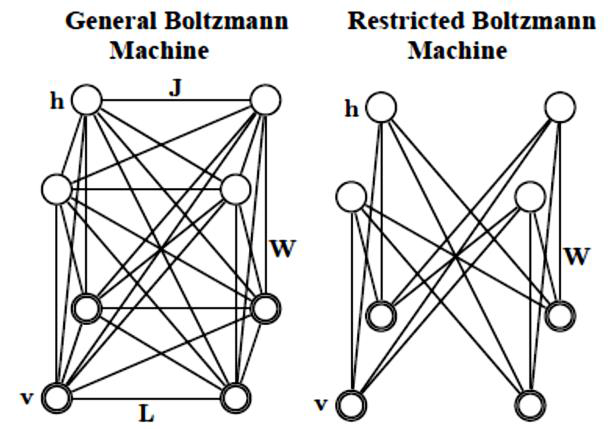
\includegraphics[width=6cm]{images/BM.png}
	 \end{column}
	\end{columns} 
  \end{frame}
  \begin{frame}
  \frametitle{Boltzman Machine}
  \begin{itemize}
		\item Energy function depends on model parameter
		\item Probability depends on weights and state of the other neurons 
		\item Unsupervised learning
		\item Used to model probability distribution:
		\begin{itemize}
		\item Apply random input
		\item Run the model for some time to generate sample from learned distribution
		\end{itemize}
		\item First used as an feature extractor
	\end{itemize}
  \end{frame}
  \subsection{Restricted Boltzmann Machines}
  \begin{frame}
    \frametitle{Restricted Boltzmann Machines}
    %\framesubtitle{A bit more information about this}
    \begin{itemize}
		\item Complete bipartite graph
		\item Stochastic neural network:
		\begin{itemize}
		\item nodes - neurons
		\item edges - synaptic connections
		\end{itemize}
	\end{itemize}
    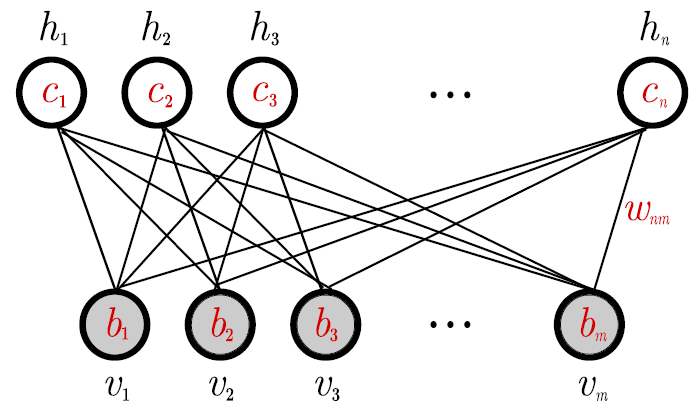
\includegraphics[width=6cm]{images/RBMnetworkGraph.png}
    %\captionof{\TINY Figure}
    \begin{itemize}
			{\TINY Source: A.Fischer, Ch.Igel: Training Restricted Boltzmann Machines: An Introduction}
    \end{itemize}
  \end{frame}
  \begin{frame}
  \frametitle{Mathematical description of  the model}
  Energy function
  \begin{align}
      \mathbf{E(v,h) = \sum_{i=1}^{V} \frac{(v_i - b_i^v)^2}{2\sigma_i^2} - \sum_{j=1}^{H} b_j^h h_j - \sum_{i=1}^{V} \sum_    {j=1}^{H} \frac{v_i}{\sigma_i} h_j w_{ij}}
  \end{align}
  Probability of (v,h)
  \begin{align}
      \mathbf{p(v,h) = \frac{e^{-E(v,h)}}{\sum_x \sum_k e^{-E(x,k)}}}
  \end{align}
  Conditional distributions
  \begin{align}
      \mathbf{p(h|v) = \sum_i{p(h_i | v)}}
  \end{align}
  \begin{align}
      \mathbf{p(h_j = 1|v) = sigm(c_j + \sum_i{W_{ji} x_i)}}
  \end{align}
  \end{frame}
  
  \subsection{Contrastive Divergence} 
  \begin{frame}
  \frametitle{Contrastive Divergence}
  \begin{itemize}
		\item Problem: Log likelihood gradient is hard to compute
		\item Run Markov chain to approximate the model distribution
		\item One step of Gibbs Sampling is sufficient
	\end{itemize}
	\begin{alertblock}{Remark}
	Training a RBM is performed by algorithm known as "Contrastive Divergence Learning"
	\end{alertblock}	
	
  \end{frame}
  \begin{frame}
  \frametitle{Contrastive Divergence  - reconstruction step}
  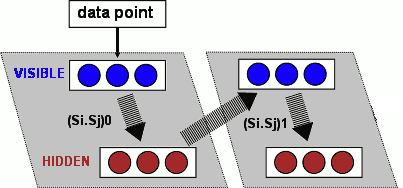
\includegraphics[width=5cm]{images/CDrecon.png}
  \begin{itemize}
		\item Get one data point from data set
		\item Use values of the data to set state of visible units - Si
		\item Compute Sj for each hidden neuron based on Si
		\item Compute (Si.Sj)0
		\item Reconstruction: on visible units compute Si using the Sj
		\item Compute state of hidden neurons Sj again using Si
		\item Use Si and Sj to compute (Si.Sj)1

	\end{itemize}
  \end{frame}
  \begin{frame}
  \frametitle{Contrastive Divergence in n steps - whole algorithm}
  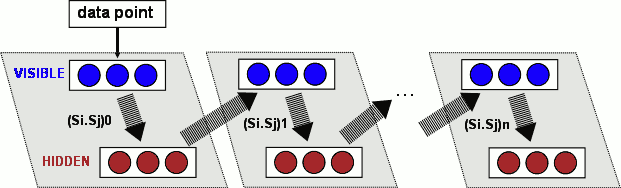
\includegraphics[width=8cm]{images/trainRBM.png}
  \begin{itemize}
		\item For each data point in data set:
		\begin{itemize}
		 \item perform reconstruction in n-steps
		 \item Accumulate CDpos = CDpos + (Si.Sj)0
		 \item Accumulate CDneg = CDneg + (Si.Sj)n
		\end{itemize}
		\item Compute average CDpos and CDneg (divide by nr of points)
		\item Compute gradient CD = CDpos - CDneg 
		\item Update weights and biases W" = W + alpha*CD
		\item Repeat for whole dataset in number of epochs (iterations)
	\end{itemize} 
  \end{frame}

  \subsection{RBM for classification} 
  \begin{frame}
  \frametitle{Using RBM for classification}
  Three approaches (Hinton):
  \begin{itemize}
		\item Use the hidden features learned by the RBM as the inputs for some standard discriminative method
		 \item Train a separate RBM on each class
		 \item Train a joint density model using a single RBM (that has two sets of visible units - y for label and x for data)
		 \begin{itemize}
		 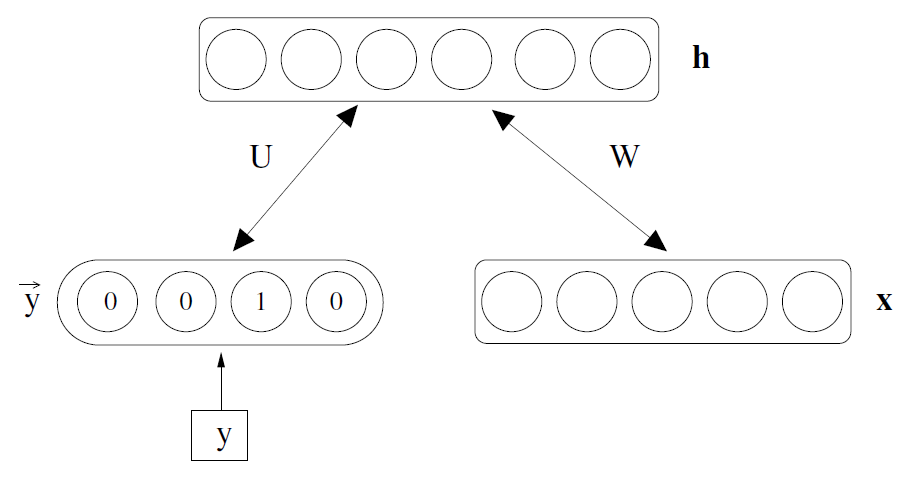
\includegraphics[width=6cm]{images/jointProbModel.png}
		 \end{itemize}
		\end{itemize}
  \end{frame}
  \section{Implementation}
  \begin{frame}
  \frametitle{Tools}
  \begin{columns}
  \begin{column}{0.5\textwidth}
  \begin{itemize}
  
\includegraphics[width=4cm]{images/python_logo.png}
  \end{itemize}
  \begin{itemize}
  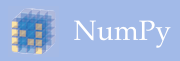
\includegraphics[width=4cm]{images/numpy_logo.png}
  \end{itemize}
  \begin{itemize}
  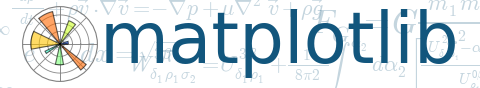
\includegraphics[width=4cm]{images/matplot_logo.png}
  \end{itemize}
  
  \end{column}
  \begin{column}{0.5\textwidth}
  \begin{itemize}
  
\includegraphics[width=6cm]{images/github_logo.png}
  \end{itemize}
  \end{column}
  \end{columns}
  \end{frame}
  \begin{frame}
  \frametitle{Data loading and preprocessing module}
  \begin{itemize}
  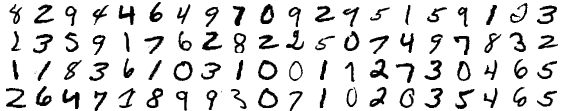
\includegraphics[width=8cm]{images/mnist.png}
  \end{itemize}
  \begin{itemize}
	\item MNIST - handwritten digit images
	\item Raw data consists of greyscale normalized images (28x28 pixels, pixel is number 0-255) and their labels (0..9)
	\item Dataset divided into training (50000), validation (10000) and test (10000) subsets 
	\item Loaded optionally from cPickle file or CSV 
	\item Data-specific, help functions implemented (binarization, transformations, scaling, visualizations)
	\end{itemize}
  \end{frame}
  \begin{frame}
  \frametitle{Generative and Discriminative models of RBM}
  \begin{columns}
        \begin{column}{0.3\textwidth}
            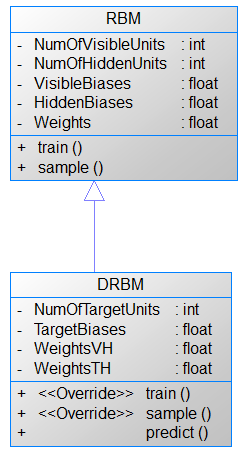
\includegraphics[width=3cm]{images/classDiagram.png}
        \end{column}
        \begin{column}{0.7\textwidth}
			\centering
			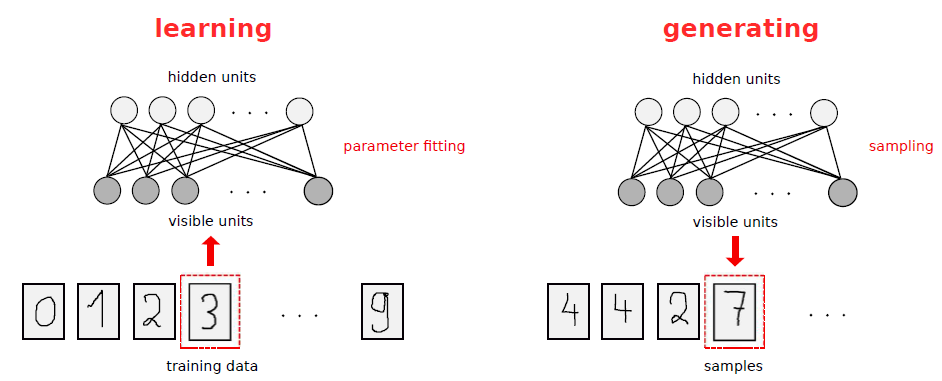
\includegraphics[width = 7cm]{images/generativeRBM.png}
			%\captionof{\TINY GRBM}
			\begin{itemize}
			{\TINY Source: A.Fischer, Ch.Igel: Training Restricted Boltzmann Machines: An Introduction}
			\end{itemize}
			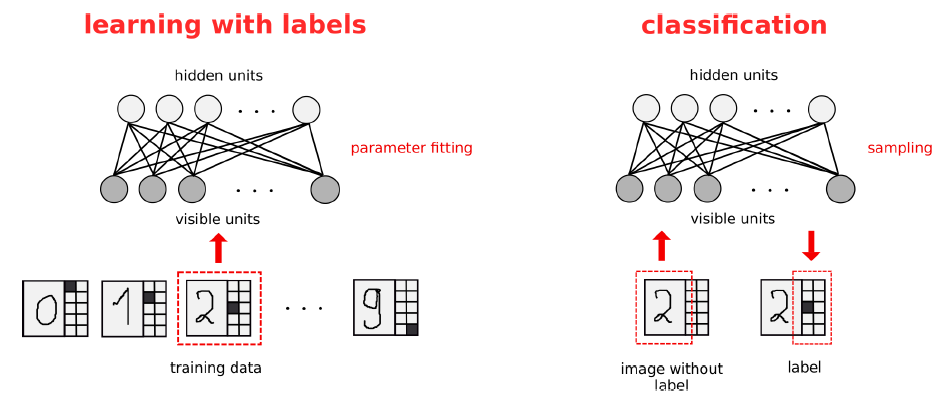
\includegraphics[width = 7cm]{images/DRBM.png}
			%\captionof{\TINY DRBM}
			\begin{itemize}
			{\TINY Source: A.Fischer, Ch.Igel: Training Restricted Boltzmann Machines: An Introduction}
			\end{itemize}
        \end{column}
    \end{columns}
  \end{frame}
   \begin{frame}
    \frametitle{Generative model - train()}
    \begin{itemize}
    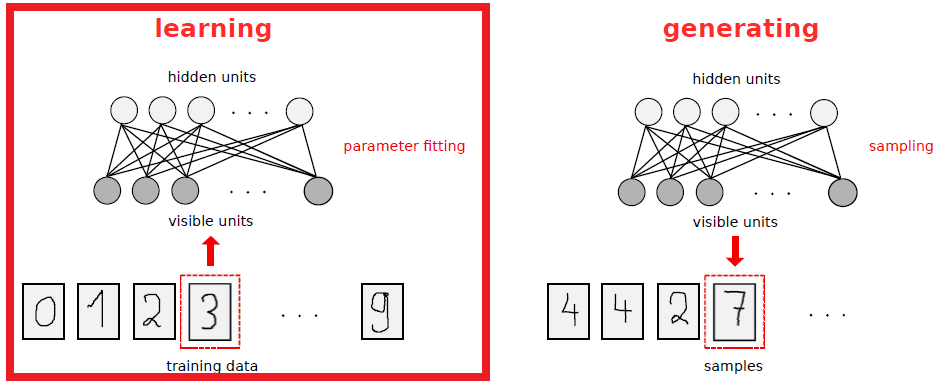
\includegraphics[width = 9cm]{images/generativeRBM_learn.png}
    \end{itemize}
    \begin{itemize}
	\item Fitting RBM parameters so that to model distribution of the training data 
	\item Iteratively performs one step of Contrastive Divergence (using Gibbs sampling) on data subset of one-class
	\item Learns until specified error threshold between data and reconstruction is reached
	\end{itemize}
	\end{frame}
	\begin{frame}
    \frametitle{Generative model - sample()}
    \begin{itemize}
    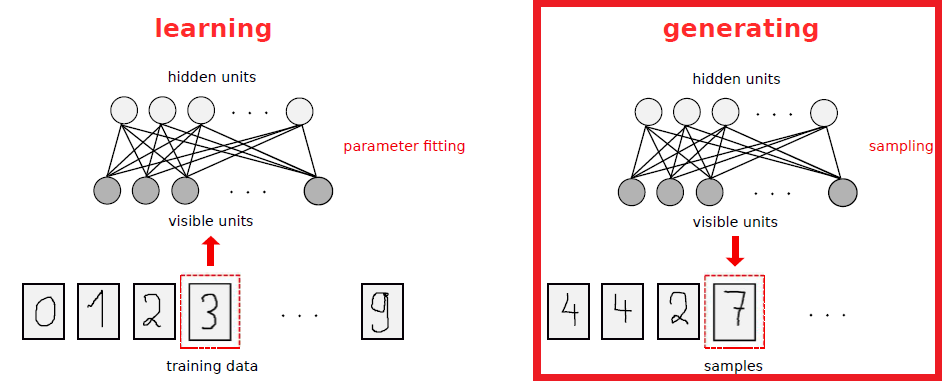
\includegraphics[width = 9cm]{images/generativeRBM_gen.png}
    \end{itemize}
    \begin{itemize}
	\item Trained RBM used to generate samples from learned distribution
	\item Shows reconstructed image for the specified digit
	\end{itemize}
	\end{frame}
  \begin{frame}
  \frametitle{Discriminative model - train()}
  \begin{columns}
   \begin{column}{0.5\textwidth}
        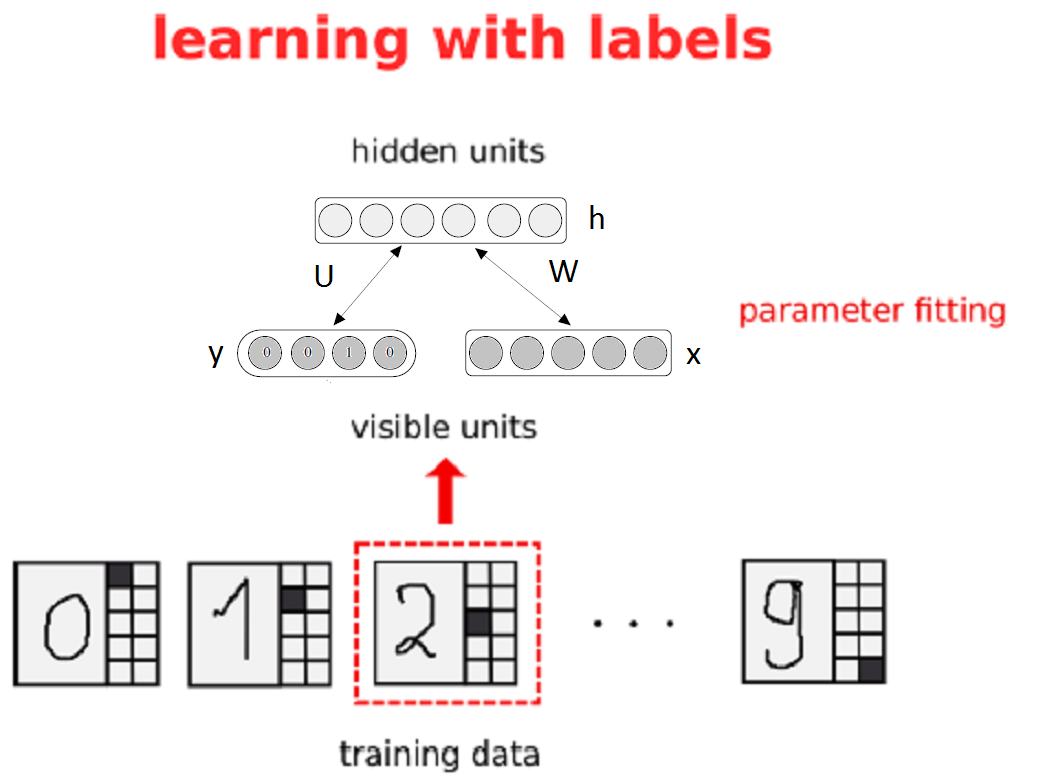
\includegraphics[width = 6cm]{images/DRBMtrain.png}
   \end{column}
  \begin{column}{0.5\textwidth}
  
  \begin{itemize}
	\item DRBM models a joint distribution of inputs (x) and target classes (y)
	\item Two sets of visible units and two weight matrices: between x and h (W) and between y and h (U)
	\item Train() performs n-step Constrastive Divergence for a mini-batch 
	\end{itemize}
\end{column}
\end{columns}
  \end{frame}
  \begin{frame}
  \frametitle{Discriminative model - predict()}
  \begin{columns}
   \begin{column}{0.4\textwidth}
        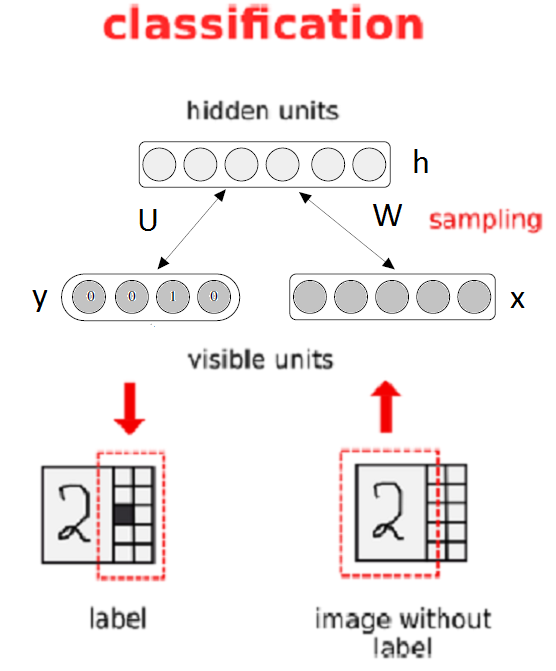
\includegraphics[width = 4cm]{images/DRBMclas.png}
   \end{column}
  \begin{column}{0.6\textwidth}
  \begin{itemize}
	\item Fix the visible variables corresponding to the image
	\item Sample target variables corresponding to the labels in chosen number of iterations
	\item For each datapoint in testset return probabilities of each class 
	\item Choose the label class with highest probability
	\item Compare with original labels
	\item Count wrong predictions and compute accuracy
	\end{itemize}
	\end{column}
\end{columns}
  \end{frame}
  \section{Results}
  \begin{frame}
  \frametitle{Testing methodology and assumptions}
  \begin{itemize}
	\item Reducing to binary problem (binarization threshold = 0.5)
	\item Parameters possible to test: 
		\begin{itemize}
		\item size of training set, 
		\item size of test set,
		\item learning rate, 
		\item initial weight distribution, 
		\item momentum, 
		\item l2 penaltization, 
		\item number of steps for contrastive divergence, 
		\item size of hidden units, 
		\item number of epochs for training, 
		\item number of iterations for sampling, 
		\item error threshold for traning, 
		\item random state
		\end{itemize}
	\end{itemize}
  \end{frame}
  
  \begin{frame}
    \frametitle{Testing generative model}
	Experiments on different sizes of hidden units
	\begin{columns}
		\begin{column}{0.15\textwidth}
            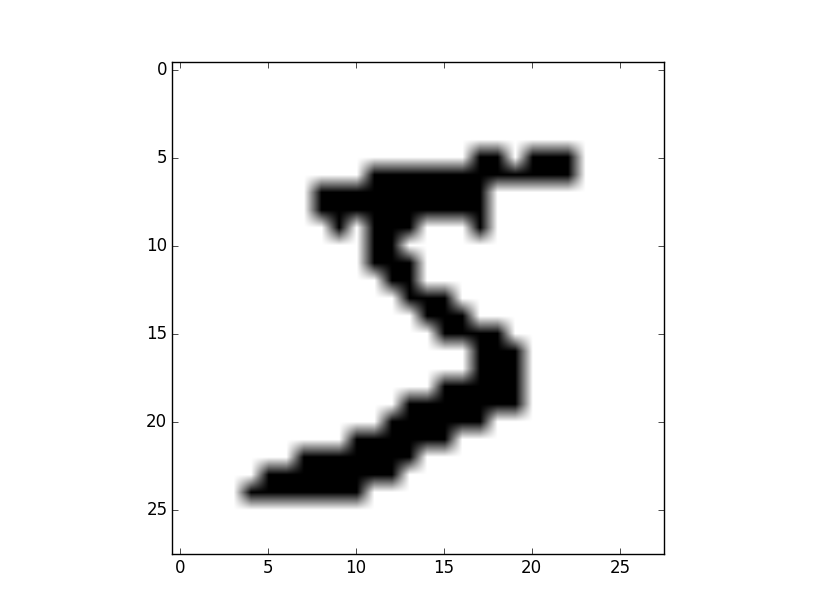
\includegraphics[width=2cm]{images/5original.png}
            \begin{itemize}
            {\TINY Original}
            \end{itemize}
		\end{column}
		\begin{column}{0.15\textwidth}
			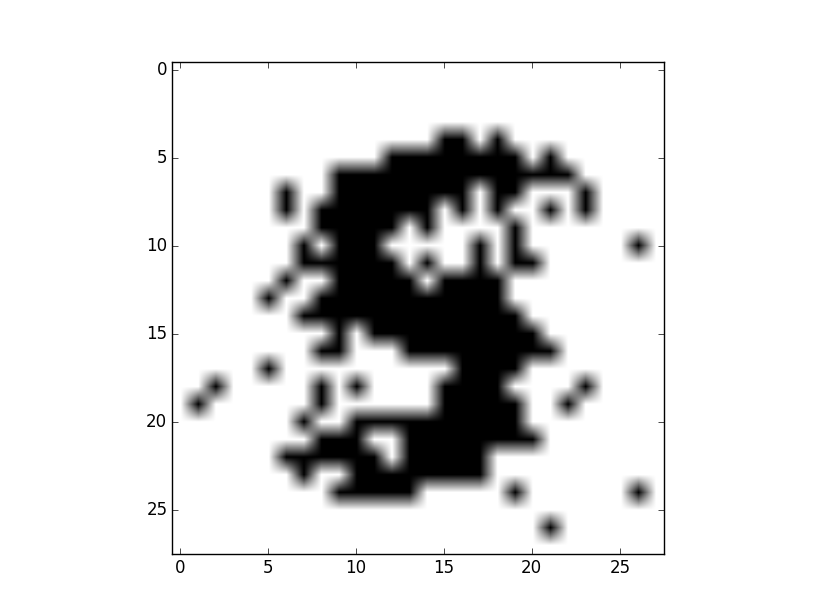
\includegraphics[width=2cm]{images/hidden200.png}
			\begin{itemize}
			{\TINY hidden=200}
			 \end{itemize}
		\end{column}
		\begin{column}{0.15\textwidth}
			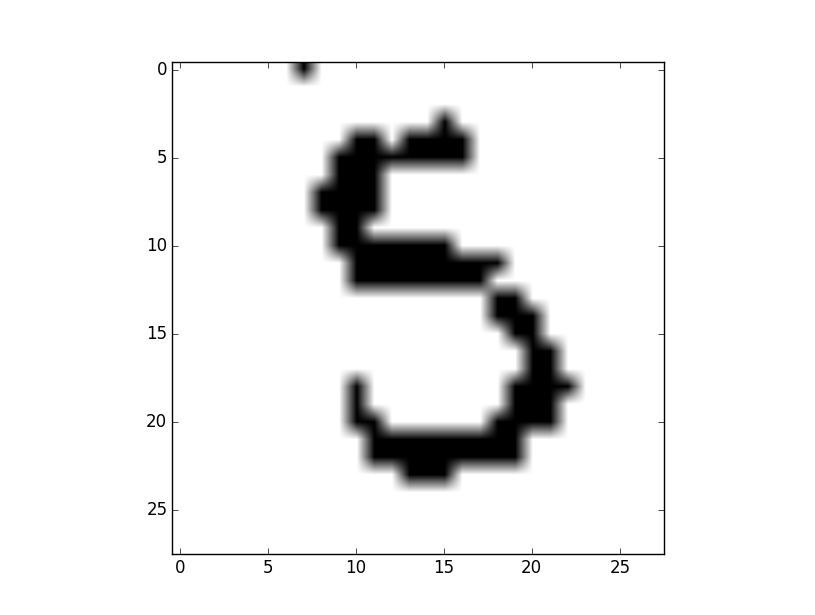
\includegraphics[width=2cm]{images/hidden300.png}
			\begin{itemize}
			{\TINY hidden=300}
			 \end{itemize}
		\end{column}
		\begin{column}{0.15\textwidth}
			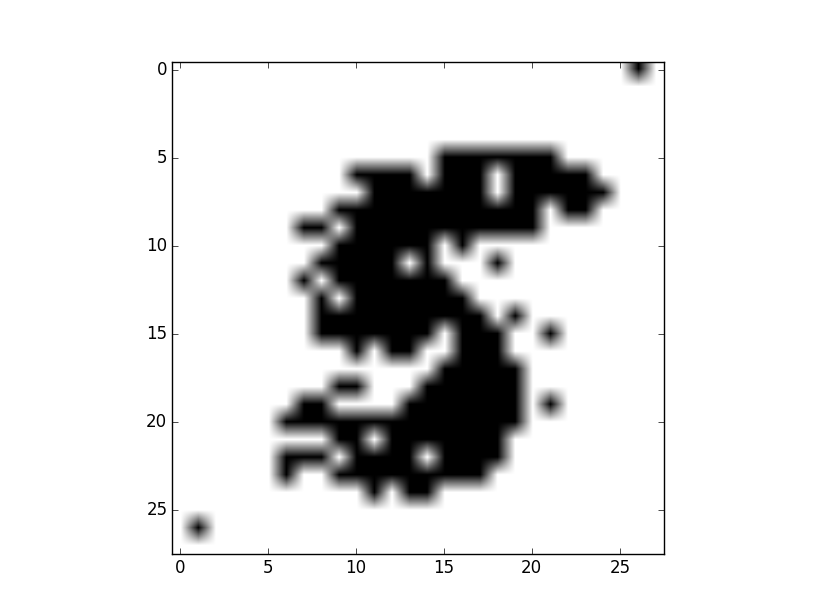
\includegraphics[width=2cm]{images/hidden400.png}
			\begin{itemize}
			{\TINY hidden=400}
			 \end{itemize}
		\end{column}
		\begin{column}{0.15\textwidth}
			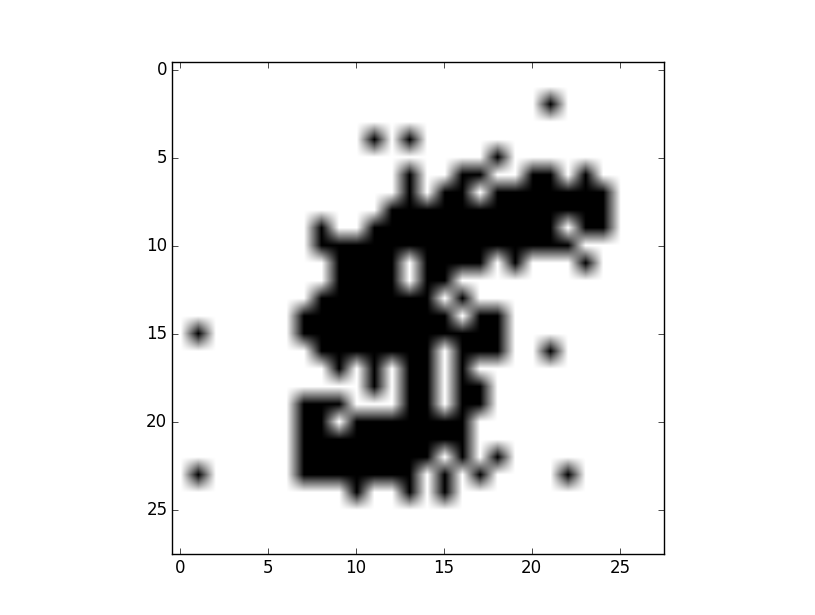
\includegraphics[width=2cm]{images/hidden500.png}
			\begin{itemize}
			{\TINY hidden=500}
			 \end{itemize}
		\end{column}
		\begin{column}{0.15\textwidth}
			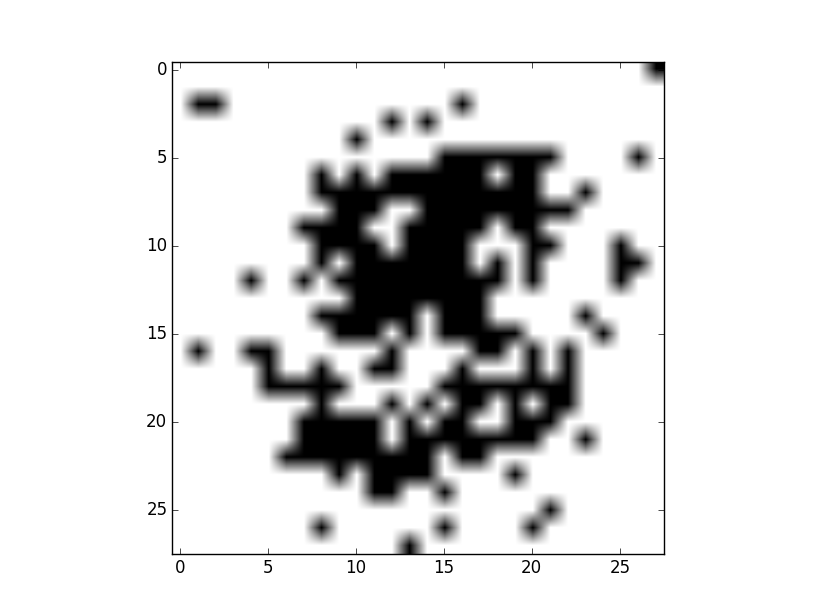
\includegraphics[width=2cm]{images/hidden700.png}
			\begin{itemize}
			{\TINY hidden=700}
			 \end{itemize}
		\end{column}
    \end{columns}

    \begin{columns}
		\begin{column}{0.15\textwidth}
            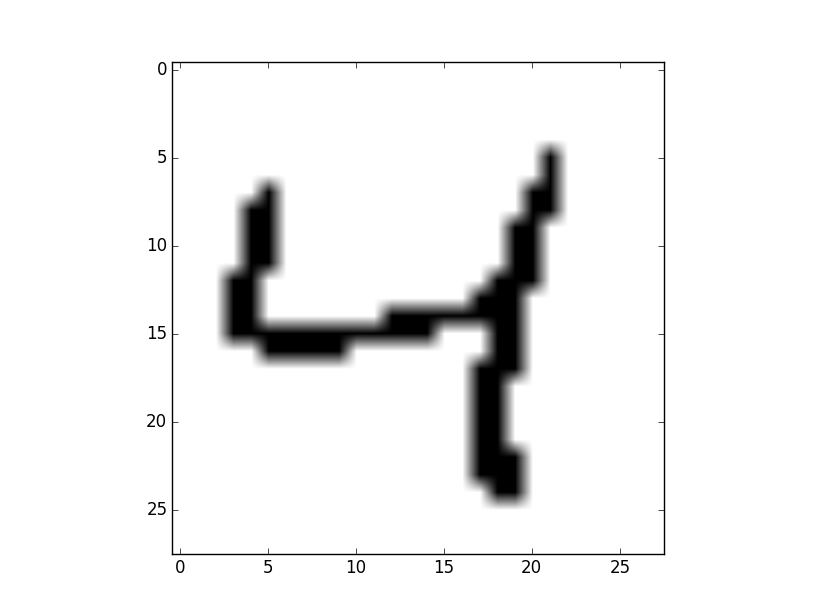
\includegraphics[width=2cm]{images/4original.png}
            \begin{itemize}
            {\TINY Original}
            \end{itemize}
		\end{column}
		\begin{column}{0.15\textwidth}
			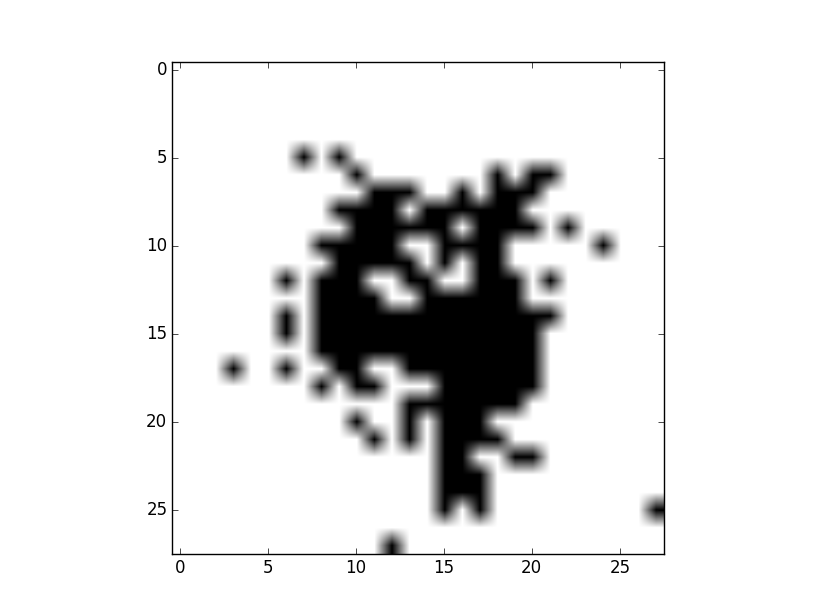
\includegraphics[width=2cm]{images/4Hidden100.png}
			\begin{itemize}
			{\TINY hidden=100}
			 \end{itemize}
		\end{column}
		\begin{column}{0.15\textwidth}
			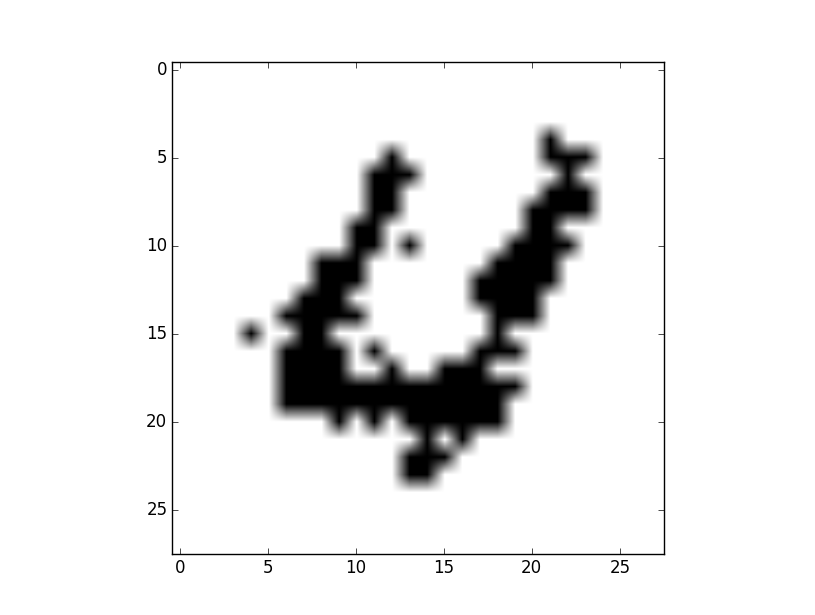
\includegraphics[width=2cm]{images/4Hidden200.png}
			\begin{itemize}
			{\TINY hidden=200}
			 \end{itemize}
		\end{column}
		\begin{column}{0.15\textwidth}
			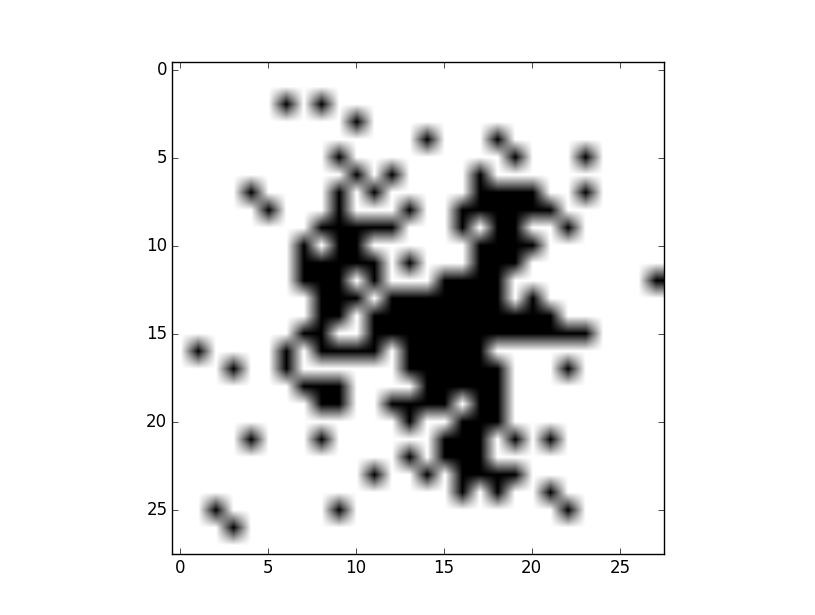
\includegraphics[width=2cm]{images/4Hidden300.png}
			\begin{itemize}
			{\TINY hidden=300}
			 \end{itemize}
		\end{column}
		\begin{column}{0.15\textwidth}
			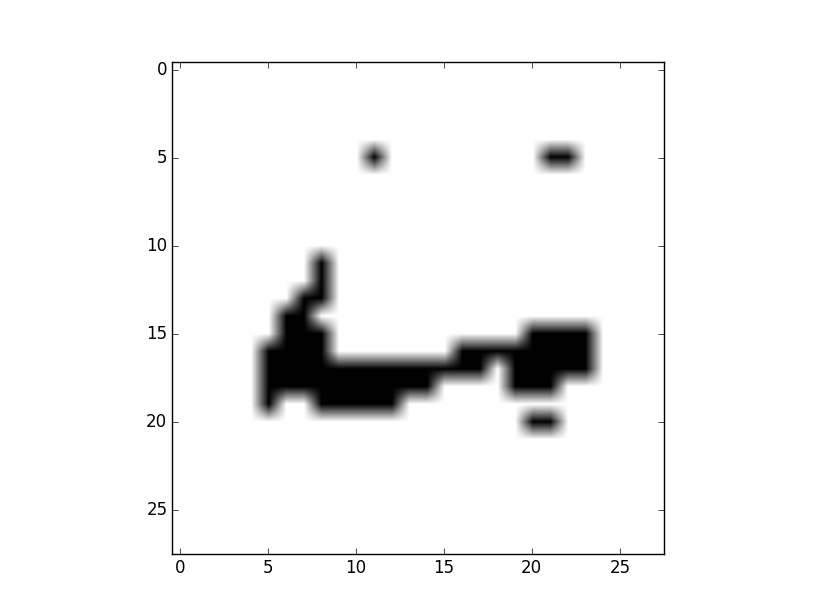
\includegraphics[width=2cm]{images/4Hidden400.png}
			\begin{itemize}
			{\TINY hidden=400}
			 \end{itemize}
		\end{column}
		\begin{column}{0.15\textwidth}
			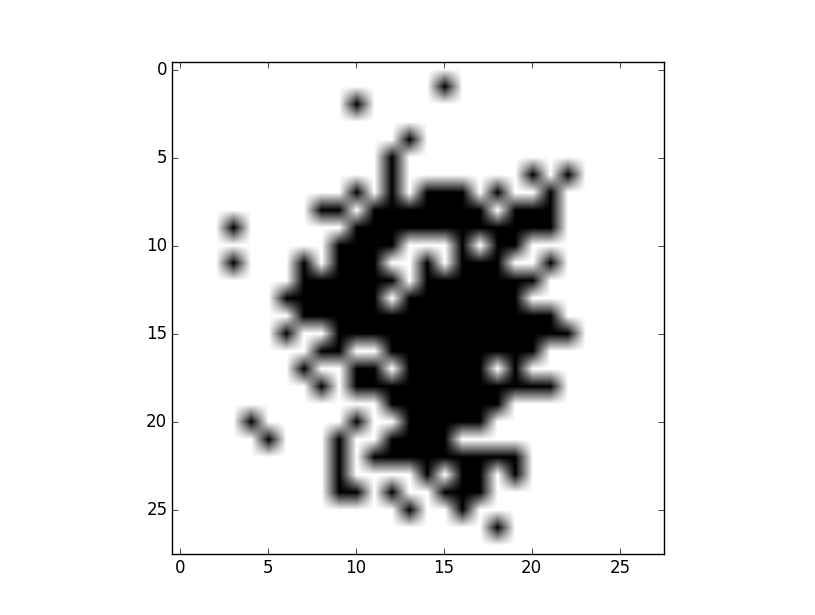
\includegraphics[width=2cm]{images/4Hidden500.png}
			\begin{itemize}
			{\TINY hidden=500}
			 \end{itemize}
		\end{column}
    \end{columns}
    \begin{alertblock}{Remark}
	Different digit classes have different optimal hyperparameters
	\end{alertblock}
  \end{frame}
  \begin{frame}
    \frametitle{Testing reconstruction with DRBM}
    \begin{itemize}
	\item Learning in mini-batches improved performance
	\item Momentum parameter for weight update other than 0.0 worsened results
	\item Optimized results for reconstruction after 500 epochs of training were good:
	\end{itemize}
	\begin{columns}
		\begin{column}{0.3\textwidth}
            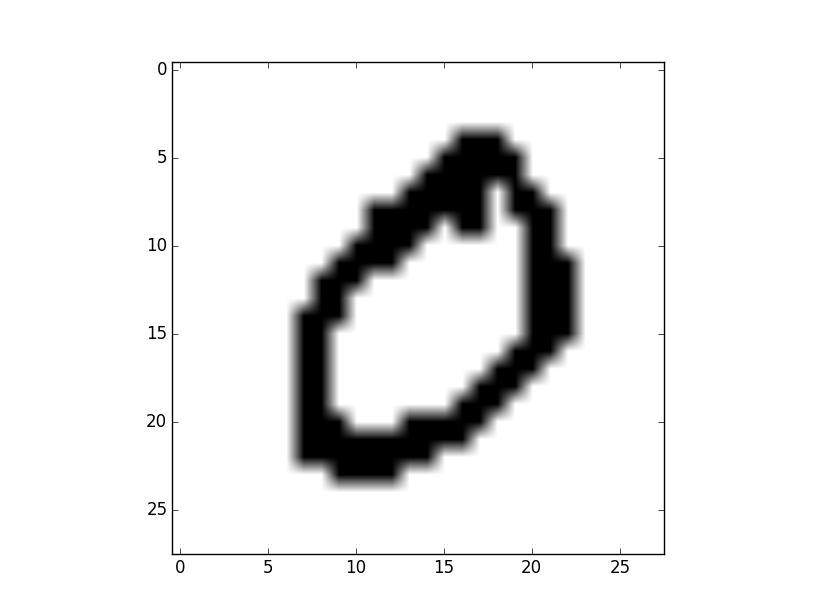
\includegraphics[width=3cm]{images/0original.png}
            \begin{itemize}
            {\TINY Original image}
            \end{itemize}
		\end{column}
		\begin{column}{0.3\textwidth}
			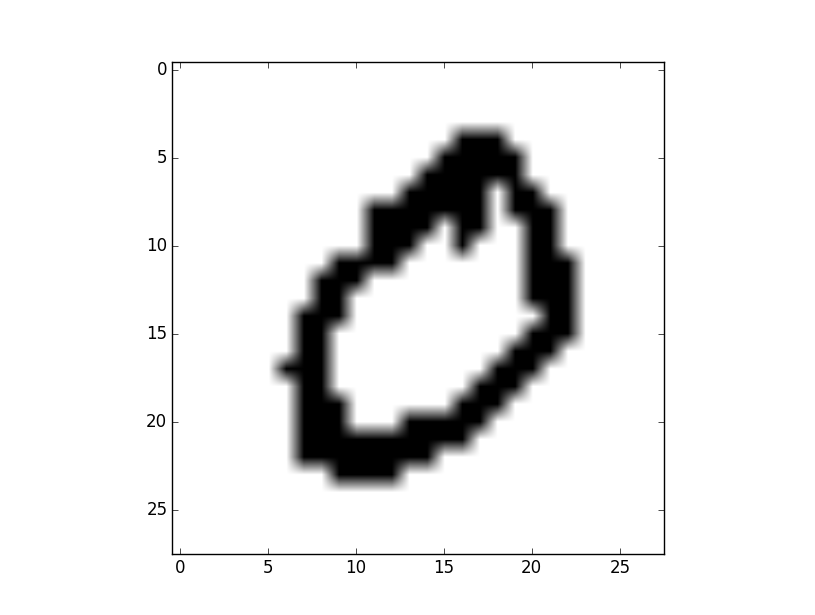
\includegraphics[width=3cm]{images/0_reconstructed_momentum00.png}
			\begin{itemize}
			{\TINY momentum=0.0}
			\end{itemize}
		\end{column}
		\begin{column}{0.3\textwidth}
			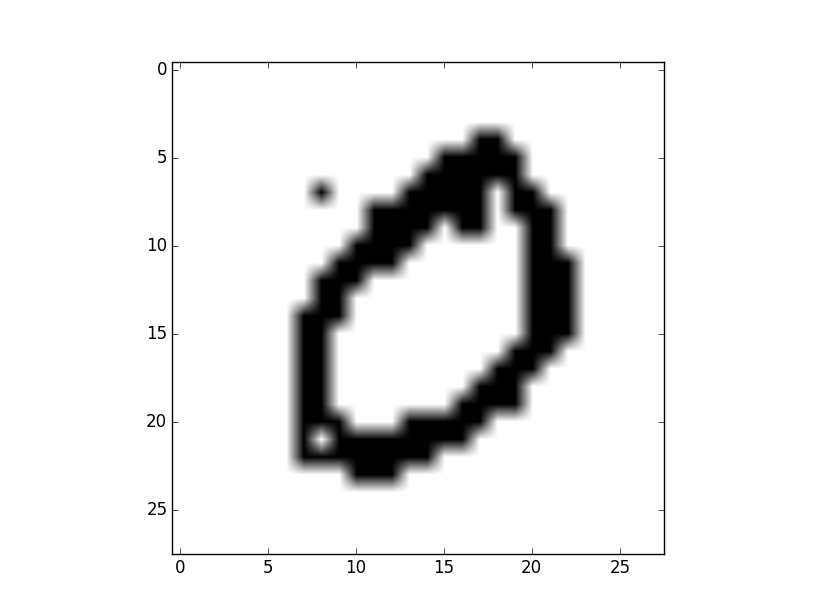
\includegraphics[width=3cm]{images/0_reconstructed_momentum05.png}
			\begin{itemize}
			{\TINY momentum=0.5}
			\end{itemize}
		\end{column}
    \end{columns}
    %{\TINY first is original, second with momentum=0.0, third with momentum=0.5}
    \begin{itemize}
    \item For 500-epoch training MSE falls below 1.0 - in about 30 minutes (on 50 train size)
    \end{itemize}
  \end{frame}
  \begin{frame}
  \frametitle{Monitoring progress of learning}
  
   \begin{columns}
		\begin{column}{0.5\textwidth}
            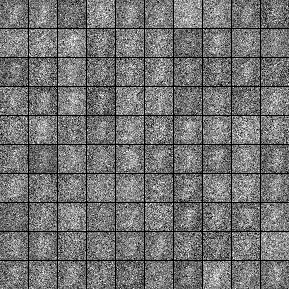
\includegraphics[width=5cm]{images/filtry_1epoch_50train.png}
		\end{column}
		\begin{column}{0.5\textwidth}
            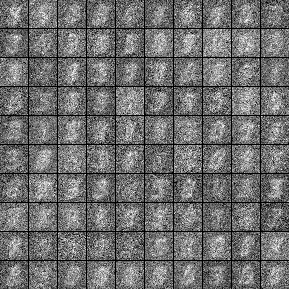
\includegraphics[width=5cm]{images/filtry_5epoch_50train.png}	
		\end{column}
    \end{columns}
    Learned weights after 1 and 5 iterations  
  \end{frame}
  \begin{frame}
  \frametitle{Monitoring progress of learning}

   \begin{columns}
		\begin{column}{0.5\textwidth}
            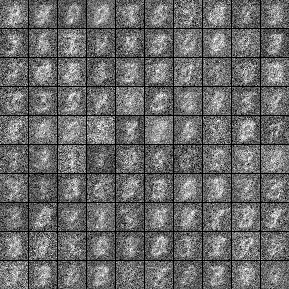
\includegraphics[width=5cm]{images/filtry_10epoch_50train.png}
		\end{column}
		\begin{column}{0.5\textwidth}
			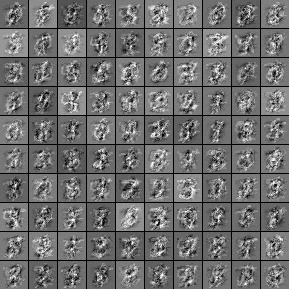
\includegraphics[width=5cm]{images/filters_epoch500_train50.png}	
		\end{column}
    \end{columns}
    Learned weights after 10 and 500 iterations
    %Learned weights after 500 iterations on 50-train dataset  
  \end{frame}
  \begin{frame}[plain]
  \frametitle{Monitoring progress of learning}
  \framesubtitle{Reconstruction error for 100 epochs}
    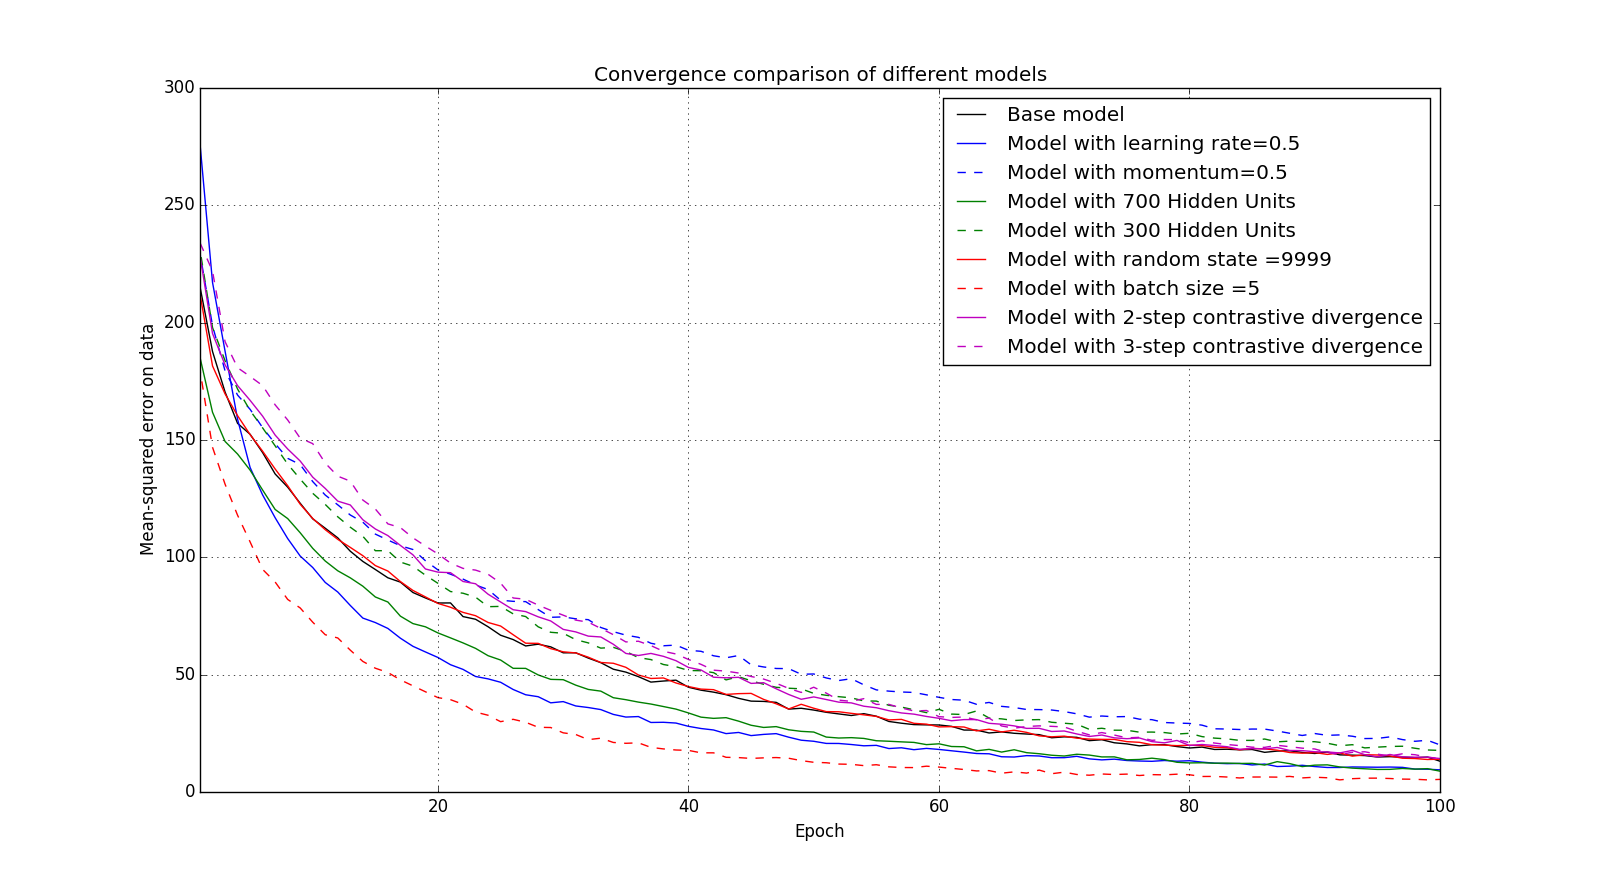
\includegraphics[width=10.5cm]{images/Plot_Convergence50train100epochs.png}
    \begin{alertblock}{Remark}
	The reconstruction error on the training set falls rapidly and consistently at the start of learning and then more slowly.
	\end{alertblock}
  \end{frame}
  \begin{frame}
  \frametitle{Model selection}
  
  \framesubtitle{Reconstruction error for first 10 epochs}
  {\TINY Base model: lr = 0.01, hidden units=500, random state =1234, batch size=10, 1-step constrastive divergence,
  no momentum}
    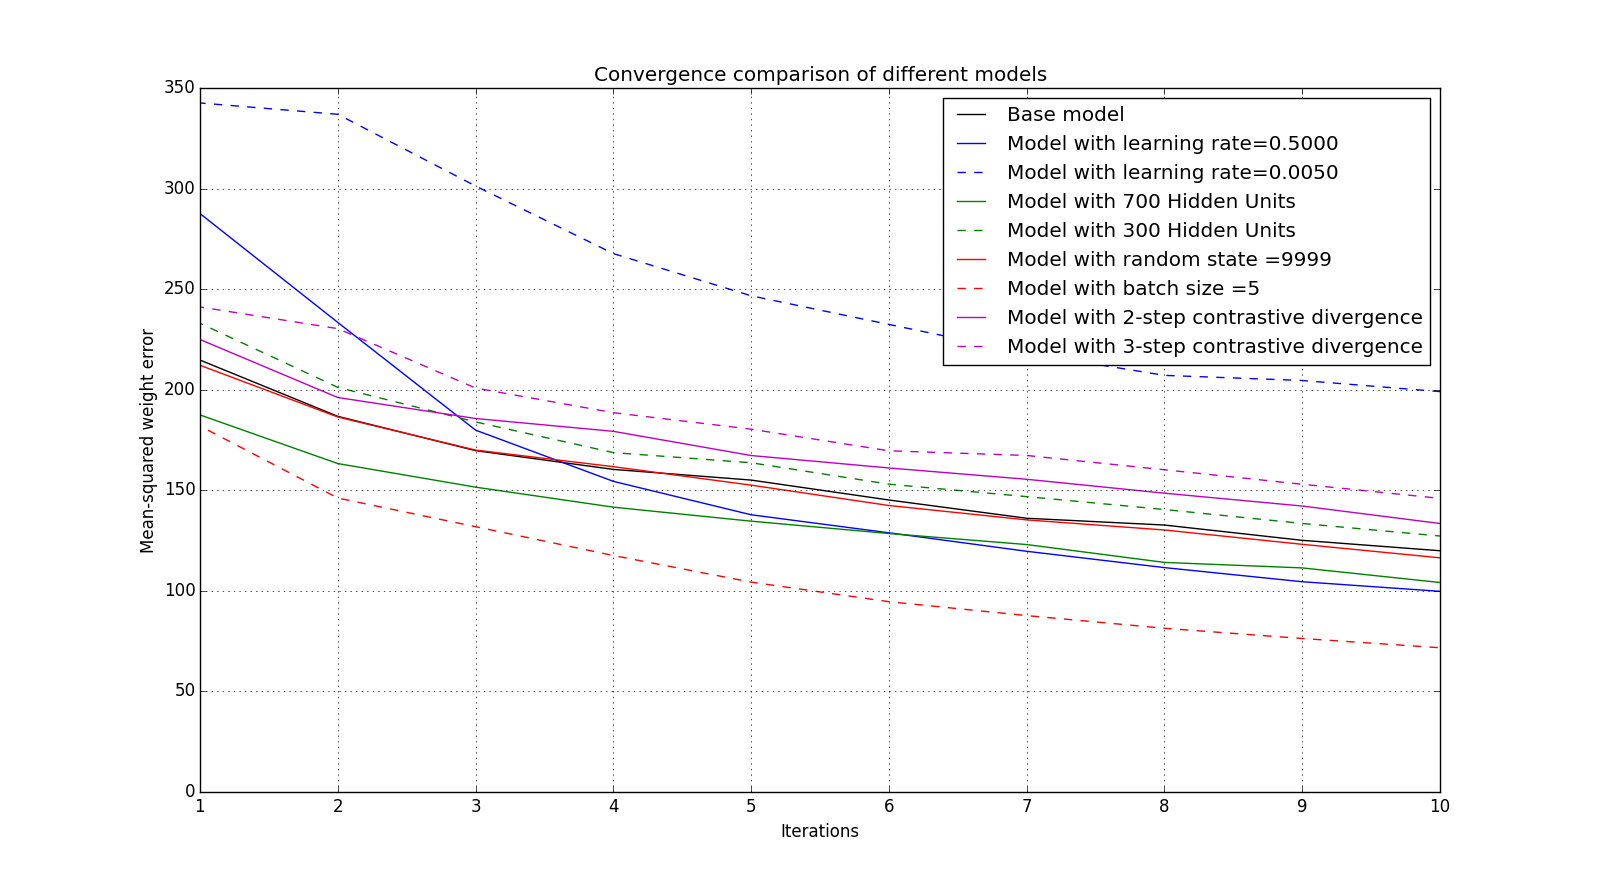
\includegraphics[width=12.5cm]{images/Plot_Convergence50train10epochs.png} 
  \end{frame}
  \begin{frame}
  \frametitle{Model selection}
  \framesubtitle{Reconstruction error for last 5 epochs}
    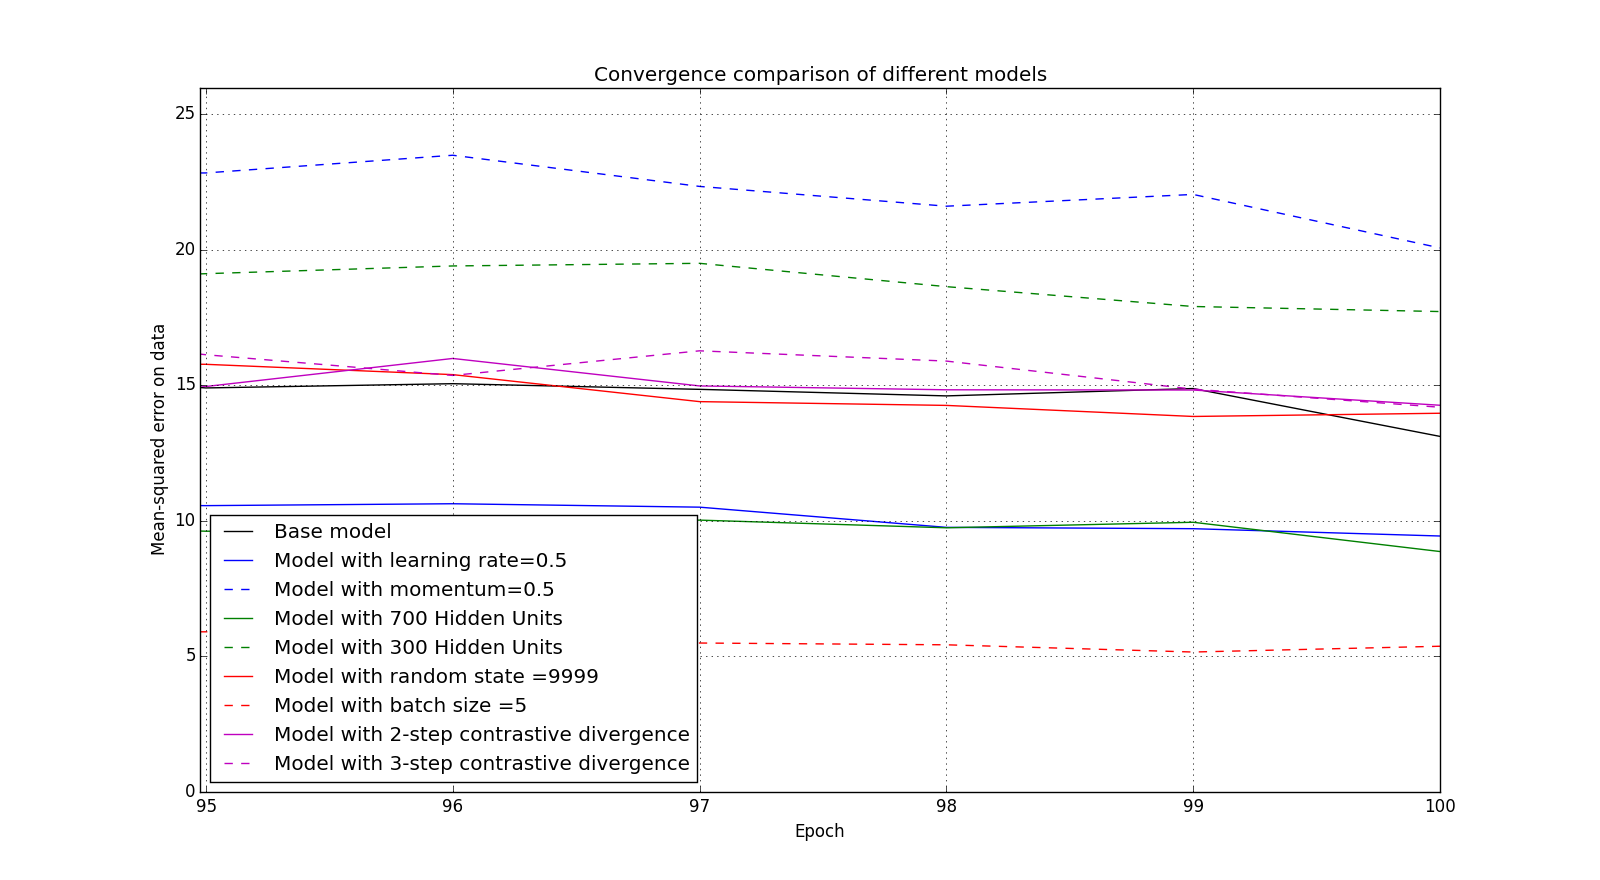
\includegraphics[width=12.5cm]{images/Plot_Convergence50train95-100epochs.png}
  \end{frame}
  \begin{frame}
    \frametitle{Model selection}
    \framesubtitle{Conclusions}
    \begin{itemize}
	\item Learning in smaller mini-batches and increasing number of hidden units (from 400 to 700) improved reconstruction
	\item However, these changes resulted in longer train time 
	\item Higher learning rate (0.5 instead of 0.05) caused reconstruction error to drop more sharply 
	\item For larger train datasets higher learning rate caused instability (after some time of drop error started to increase)
	\item Different random states do not change reconstruction error significantly
	\item 1-step contrastive divergence is optimal
	\end{itemize}
  \end{frame} 
  \begin{frame}
    \frametitle{Testing RBM for classification (I)}
    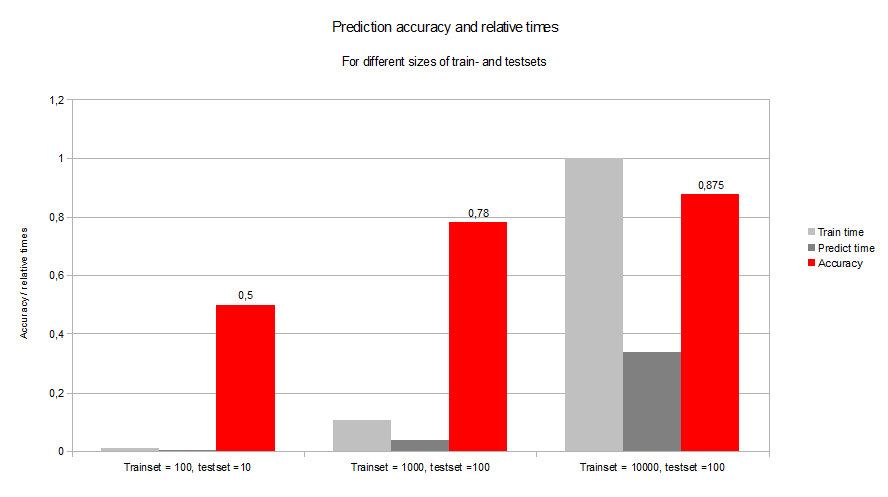
\includegraphics[width=9.5cm]{images/acc2.png}
    \begin{itemize}
	\item Classification accuracy depends on are train- and test sets size
	\item For larger data sets train and prediction times become prohibitive for personal computing 
	\end{itemize}
  \end{frame}
  \begin{frame}
    \frametitle{Testing RBM for classification(II)}
    \begin{itemize}
    \item Optimal hyperparameters for training phase were chosen
	\item Performing 100 percent accurate classification on training data could be achieved even on small sets
	\item Classification accuracy on new data achieved so far is 95 percent (MNIST 50000 trainset and 10000-validation set)
	\item Better results are expected given greater computing power
	\begin{block}{Conclusion}
	Implementation and tests on synthetic data within this project proved that RBMs can be effectively used as standalone classifiers. 
	\end{block}
	\end{itemize}
  \end{frame}
  \section{Further work}
  \begin{frame}
    \frametitle{Plans for further work}
    \begin{itemize}
    \item Test-against-all-labels prediction approach
    \item Optimizing algorithms for best performance
	\item Testing on gaussian values
	\item Another dataset, possibly CIFAR
	\end{itemize}
  \end{frame}
  \begin{frame}[allowframebreaks]
  \frametitle<presentation>{Literature}    
  \begin{thebibliography}{10}    
  %\beamertemplatebookbibitems
  %\bibitem{Autor1990}
    %A.~Autor.
    %\newblock {\em Introduction to Giving Presentations}.
    %\newblock Klein-Verlag, 1990.
  \beamertemplatearticlebibitems
  \bibitem{Larochelle}
    Hugo Larochelle, Yoshua Bengio.
    \newblock Classification using Discriminative Restricted Boltzmann Machines.
    \newblock {\em Proceedings of the 25th International Conference on Machine Learning}, 2008.
   \bibitem{Hinton}
    Geoffrey Hinton.
    \newblock A Pratical Guide to Training Restricted Boltzmann Machines.
    \newblock {\em UTML TR 2010-003}, 2010.
   \bibitem {Miguel}
	Miguel A. Carreira-Perpin�n, Geoffrey E. Hinton 
	\newblock On Contrastive Divergence Learning
	\newblock {\em Artificial Intelligence and Statistics}, 2005.
   %\bibitem{Fischer}
    %Asja Fischer, Christian Igel.
    %\newblock Training Restricted Boltzmann Machines: An Introduction.
    %\newblock {\em UTML TR 2010-003}, 2(1):50--100, 2008.
  \end{thebibliography}
  \end{frame}
  \begin{frame}[plain]
  \frametitle{Thank you}
  \includegraphics[width=11cm]{images/qa.png}
  \end{frame}
\end{document}
